\documentclass[11pt,a4paper]{article}

% --- Packages ---
\usepackage[utf8]{inputenc}
\usepackage[T1]{fontenc}
\usepackage{lmodern}
\usepackage[margin=2.5cm]{geometry}
\usepackage{amsmath,amssymb}
\usepackage{booktabs}
\usepackage{array}
\usepackage{tabularx}
\usepackage{enumitem}
\usepackage{xcolor}
\usepackage{tcolorbox}
\usepackage{fancyhdr}
\usepackage{titlesec}
\usepackage{hyperref}
\usepackage{graphicx}
\usepackage{listings}
\usepackage{tikz}
\usetikzlibrary{arrows.meta,positioning,calc,decorations.pathreplacing}

% --- Colors ---
\definecolor{alfaisalgreen}{RGB}{46,125,50}
\definecolor{lightgreen}{RGB}{232,245,233}
\definecolor{darkgray}{RGB}{60,60,60}
\definecolor{questionblue}{RGB}{21,101,192}
\definecolor{lightblue}{RGB}{227,242,253}
\definecolor{warnorange}{RGB}{230,126,34}
\definecolor{lightorange}{RGB}{255,243,224}
\definecolor{codegray}{RGB}{245,245,245}

% --- tcolorbox styles ---
\tcbset{
    intuitionbox/.style={
        colback=lightgreen,
        colframe=alfaisalgreen,
        fonttitle=\bfseries,
        title=#1,
        arc=2mm,
        boxrule=0.8pt,
        left=6pt,right=6pt,top=4pt,bottom=4pt
    },
    questionbox/.style={
        colback=lightblue,
        colframe=questionblue,
        fonttitle=\bfseries,
        title=#1,
        arc=2mm,
        boxrule=0.8pt,
        left=6pt,right=6pt,top=4pt,bottom=4pt
    },
    warnbox/.style={
        colback=lightorange,
        colframe=warnorange,
        fonttitle=\bfseries,
        title=#1,
        arc=2mm,
        boxrule=0.8pt,
        left=6pt,right=6pt,top=4pt,bottom=4pt
    }
}

% --- Code listing style ---
\lstset{
    backgroundcolor=\color{codegray},
    basicstyle=\ttfamily\small,
    breaklines=true,
    frame=single,
    rulecolor=\color{gray!40},
    xleftmargin=6pt,
    xrightmargin=6pt,
    aboveskip=8pt,
    belowskip=8pt
}

% --- Header/Footer ---
\pagestyle{fancy}
\fancyhf{}
\fancyhead[L]{\small\textcolor{darkgray}{MAI554 -- Deep Learning for NLP}}
\fancyhead[R]{\small\textcolor{darkgray}{Lecture 4 Notes}}
\fancyfoot[C]{\small\textcolor{darkgray}{\thepage}}
\renewcommand{\headrulewidth}{0.4pt}

% --- Section formatting ---
\titleformat{\section}{\Large\bfseries\color{alfaisalgreen}}{}{0em}{}[\vspace{-4pt}\textcolor{alfaisalgreen}{\rule{\textwidth}{0.8pt}}]
\titleformat{\subsection}{\large\bfseries\color{darkgray}}{}{0em}{}

% --- Document ---
\begin{document}

% ============================================================
% TITLE PAGE
% ============================================================
\begin{titlepage}
\centering
\vspace*{3cm}

{\Huge\bfseries\color{alfaisalgreen} Lecture 4}\\[0.8cm]
{\LARGE\bfseries From Word Embedding to\\[0.3cm] Contextual Embedding\\[0.3cm] using RNN, LSTM, and GRU}\\[1.5cm]

{\Large\textbf{Lecture Notes}}\\[0.5cm]
{\large MAI554 -- Deep Learning for NLP}\\[2cm]

{\large\textbf{Prof.\ Anis Koubaa}}\\[0.3cm]
{\normalsize College of Engineering, Alfaisal University}\\[0.2cm]
{\normalsize\texttt{akoubaa@alfaisal.edu}}\\[3cm]

{\normalsize Spring 2025}

\vfill
\end{titlepage}

% ============================================================
% HOW TO USE
% ============================================================
\section*{How to Use These Notes}

These notes distill the key ideas from Lecture~4 into a logical flow. Each section follows a pattern: \textbf{intuition first, then math, then a concrete example}. Self-check questions appear throughout the text. Full solutions are collected in the Appendix.

\tableofcontents
\newpage

% ============================================================
% 1. THE BIG PICTURE
% ============================================================
\section{The Big Picture: Why Contextual Embeddings?}

\subsection{The Problem with Static Embeddings}

In Lecture~3, we studied \textbf{static embeddings} (Word2Vec, GloVe, fastText). They map each word to a \emph{single fixed vector}, regardless of context. Consider the word \textbf{``bank''}:

\begin{itemize}[leftmargin=1.5em]
    \item \textit{``The bank by the river''} --- refers to a riverbank (nature)
    \item \textit{``The bank in the city''} --- refers to a financial institution
\end{itemize}

With static embeddings, ``bank'' gets \textbf{the same vector} in both sentences. The model cannot distinguish between these two meanings.

\begin{tcolorbox}[intuitionbox={Key Insight}]
We need a representation where the \textbf{same word gets different vectors} depending on the surrounding words. This is what \textbf{contextual embeddings} achieve, and RNNs are the mechanism that makes it possible.
\end{tcolorbox}

\subsection{The Journey Ahead}

\begin{center}
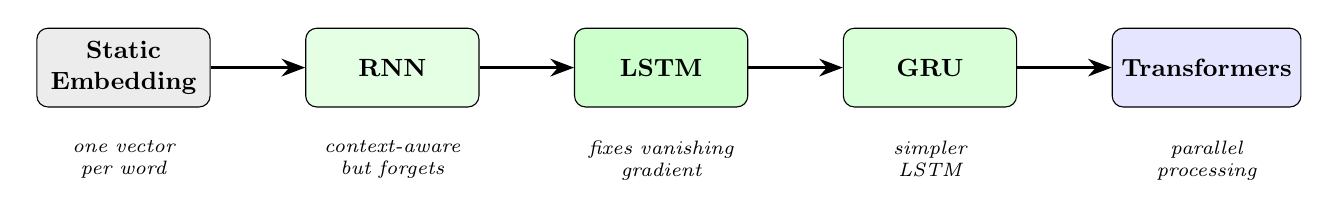
\begin{tikzpicture}[
    node distance=1.2cm,
    box/.style={draw, rounded corners, minimum height=1cm, minimum width=2.2cm, font=\small\bfseries, align=center},
    arr/.style={-{Stealth[length=3mm]}, thick}
]
\node[box, fill=gray!15] (static) {Static\\Embedding};
\node[box, fill=green!10, right=of static] (rnn) {RNN};
\node[box, fill=green!20, right=of rnn] (lstm) {LSTM};
\node[box, fill=green!15, right=of lstm] (gru) {GRU};
\node[box, fill=blue!10, right=of gru] (trans) {Transformers};

\draw[arr] (static) -- (rnn);
\draw[arr] (rnn) -- (lstm);
\draw[arr] (lstm) -- (gru);
\draw[arr] (gru) -- (trans);

\node[below=0.3cm, font=\scriptsize\itshape, text width=2.2cm, align=center] at (static.south) {one vector\\per word};
\node[below=0.3cm, font=\scriptsize\itshape, text width=2.2cm, align=center] at (rnn.south) {context-aware\\but forgets};
\node[below=0.3cm, font=\scriptsize\itshape, text width=2.2cm, align=center] at (lstm.south) {fixes vanishing\\gradient};
\node[below=0.3cm, font=\scriptsize\itshape, text width=2.2cm, align=center] at (gru.south) {simpler\\LSTM};
\node[below=0.3cm, font=\scriptsize\itshape, text width=2.2cm, align=center] at (trans.south) {parallel\\processing};
\end{tikzpicture}
\end{center}

Each architecture solves a limitation of the previous one.

% ============================================================
% 2. TEXT PRE-PROCESSING
% ============================================================
\section{Text Pre-Processing Pipeline}

Before any model can process text, raw text must be converted into numerical vectors. The pipeline has \textbf{6 steps}:

\begin{center}
\begin{tikzpicture}[
    step/.style={draw, rounded corners, fill=alfaisalgreen!10, minimum height=0.8cm, minimum width=1.8cm, font=\small, align=center},
    arr/.style={-{Stealth[length=2.5mm]}, thick, alfaisalgreen}
]
\node[step] (s1) {1.~Clean};
\node[step, right=0.4cm of s1] (s2) {2.~Stem};
\node[step, right=0.4cm of s2] (s3) {3.~Tokenize};
\node[step, right=0.4cm of s3] (s4) {4.~Index};
\node[step, right=0.4cm of s4] (s5) {5.~Pad};
\node[step, right=0.4cm of s5] (s6) {6.~Embed};

\draw[arr] (s1) -- (s2);
\draw[arr] (s2) -- (s3);
\draw[arr] (s3) -- (s4);
\draw[arr] (s4) -- (s5);
\draw[arr] (s5) -- (s6);
\end{tikzpicture}
\end{center}

\textbf{Worked example:} Input = \texttt{"I love NLP! Processing123 running"}

\begin{center}
\begin{tabular}{@{}clp{8cm}@{}}
\toprule
\textbf{Step} & \textbf{Operation} & \textbf{Result} \\
\midrule
1 & Clean (numbers, special chars, lowercase) & \texttt{"i love nlp processing running"} \\
2 & Stem (reduce to root forms) & \texttt{"i love nlp process run"} \\
3 & Tokenize (split) & \texttt{[i, love, nlp, process, run]} \\
4 & Index (map to integers) & \texttt{[10, 357, 962, 445, 223]} \\
5 & Pad (fix length to 6) & \texttt{[10, 357, 962, 445, 223, 0]} \\
6 & Embed (index $\to$ vector) & Each index $\to$ dense vector, e.g.\ dim=4 \\
\bottomrule
\end{tabular}
\end{center}

\subsection{Why Padding?}

Neural networks process data in \textbf{batches}. All sequences in a batch must have the \textbf{same length}. Padding adds zeros to shorter sequences so they match the longest one. This enables parallel processing (1$\times$ speed) vs.\ sequential processing ($N\times$ slower).

\subsection{What is Masking?}

Padding tokens are meaningless. \textbf{Masking} tells the model to ignore them:

\begin{lstlisting}[language=Python]
mask = (sequence != 0)              # True for real tokens, False for padding
output = process(sequence * mask)   # Padded positions contribute nothing
\end{lstlisting}

Without masking, the model wastes computation on zeros and may learn incorrect patterns.

\begin{tcolorbox}[questionbox={Self-Check Q1}]
Why can't we simply feed variable-length sequences to an RNN without padding? \textit{(Solution in Appendix)}
\end{tcolorbox}

% ============================================================
% 3. RNN
% ============================================================
\section{Recurrent Neural Networks (RNN)}

\subsection{From Feed-Forward to Recurrence}

\textbf{Feed-forward networks} process each input independently---there is no memory of previous inputs. This is fine for tasks like image classification, but language is \textbf{sequential}: the meaning of a word depends on what came before.

\begin{center}
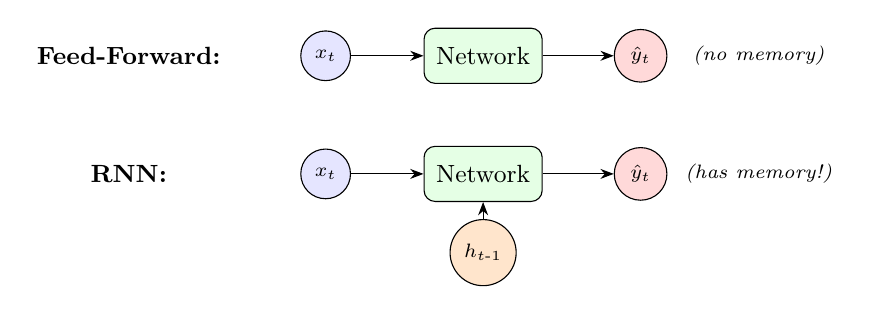
\begin{tikzpicture}[
    box/.style={draw, rounded corners, fill=green!10, minimum height=0.7cm, minimum width=1.5cm, font=\small},
    lbl/.style={font=\small}
]
% Feed-forward
\node[lbl, font=\small\bfseries] at (-2.5, 1.5) {Feed-Forward:};
\node[circle, draw, fill=blue!10, minimum size=0.6cm, font=\scriptsize] (x1) at (0, 1.5) {$x_t$};
\node[box] (nn1) at (2, 1.5) {Network};
\node[circle, draw, fill=red!15, minimum size=0.6cm, font=\scriptsize] (y1) at (4, 1.5) {$\hat{y}_t$};
\draw[-{Stealth}] (x1) -- (nn1);
\draw[-{Stealth}] (nn1) -- (y1);
\node[lbl, font=\scriptsize\itshape] at (5.5, 1.5) {(no memory)};

% RNN
\node[lbl, font=\small\bfseries] at (-2.5, 0) {RNN:};
\node[circle, draw, fill=blue!10, minimum size=0.6cm, font=\scriptsize] (x2) at (0, 0) {$x_t$};
\node[box] (nn2) at (2, 0) {Network};
\node[circle, draw, fill=red!15, minimum size=0.6cm, font=\scriptsize] (y2) at (4, 0) {$\hat{y}_t$};
\draw[-{Stealth}] (x2) -- (nn2);
\draw[-{Stealth}] (nn2) -- (y2);
\node[circle, draw, fill=orange!20, minimum size=0.6cm, font=\scriptsize] (h) at (2, -1) {$h_{t\text{-}1}$};
\draw[-{Stealth}] (h) -- (nn2);
\node[lbl, font=\scriptsize\itshape] at (5.5, 0) {(has memory!)};
\end{tikzpicture}
\end{center}

The key innovation is the \textbf{hidden state} $h_t$, which acts as \textbf{memory} passed from one time step to the next.

\subsection{The RNN Equation}

At each time step $t$, the RNN computes:

\begin{equation}
\boxed{h_t = \tanh(W_h \cdot h_{t-1} + W_x \cdot x_t + b)}
\end{equation}

\begin{center}
\begin{tabular}{@{}cl@{}}
\toprule
\textbf{Symbol} & \textbf{Meaning} \\
\midrule
$x_t \in \mathbb{R}^m$ & Current input (word embedding at time $t$) \\
$h_{t-1} \in \mathbb{R}^n$ & Previous hidden state (memory from past words) \\
$W_x \in \mathbb{R}^{n \times m}$ & Input weight matrix \\
$W_h \in \mathbb{R}^{n \times n}$ & Hidden state weight matrix (recurrent weights) \\
$b \in \mathbb{R}^n$ & Bias vector \\
$\tanh$ & Squashes output to $[-1, +1]$ \\
\bottomrule
\end{tabular}
\end{center}

\begin{tcolorbox}[intuitionbox={Intuition}]
Think of the hidden state as a person reading a sentence word by word. After each word, they update their mental summary. By the end, $h_T$ contains a summary of the \textbf{entire sequence}.
\end{tcolorbox}

\subsection{Worked Example: Sentiment Analysis of ``I like AI''}

Let us trace through an RNN processing the sentence ``I like AI'' with hidden size = 3.

\medskip\noindent\textbf{Setup:}

\[
W_x = \begin{bmatrix} 0.1 & 0.2 & 0.3 \\ 0.2 & 0.3 & 0.1 \\ 0.3 & 0.1 & 0.2 \end{bmatrix}, \quad
W_h = \begin{bmatrix} 0.2 & 0.1 & 0.1 \\ 0.1 & 0.2 & 0.1 \\ 0.1 & 0.1 & 0.2 \end{bmatrix}, \quad
b = \begin{bmatrix} 0.1 \\ 0.1 \\ 0.1 \end{bmatrix}
\]

Word embeddings (dim=3): $x_I = [0.2, -0.1, 0.4]$,\; $x_{\text{like}} = [0.8, 0.6, 0.3]$,\; $x_{\text{AI}} = [0.5, 0.4, 0.2]$

Initial hidden state: $h_0 = [0, 0, 0]$

\medskip
\begin{tcolorbox}[colback=white, colframe=alfaisalgreen, boxrule=0.5pt, title={\textbf{Step 1 --- Processing ``I''}}]
\[
W_x \cdot x_I + W_h \cdot h_0 + b = [0.15,\; 0.25,\; 0.35]
\]
\[
h_1 = \tanh([0.15,\; 0.25,\; 0.35]) = [-0.05,\; 0.10,\; 0.20]
\]
The hidden state now encodes information about the word ``I''.
\end{tcolorbox}

\begin{tcolorbox}[colback=white, colframe=alfaisalgreen, boxrule=0.5pt, title={\textbf{Step 2 --- Processing ``like''}}]
Using $h_1 = [-0.05, 0.10, 0.20]$ as memory:
\[
W_x \cdot x_{\text{like}} + W_h \cdot h_1 + b = [0.35,\; 0.25,\; -0.15]
\]
\[
h_2 = \tanh([0.35,\; 0.25,\; -0.15]) = [0.30,\; 0.20,\; -0.10]
\]
Now $h_2$ encodes information about both ``I'' and ``like''.
\end{tcolorbox}

\begin{tcolorbox}[colback=white, colframe=alfaisalgreen, boxrule=0.5pt, title={\textbf{Step 3 --- Processing ``AI''}}]
Using $h_2 = [0.30, 0.20, -0.10]$ as memory:
\[
W_x \cdot x_{\text{AI}} + W_h \cdot h_2 + b = [0.45,\; 0.15,\; 0.30]
\]
\[
h_3 = \tanh([0.45,\; 0.15,\; 0.30]) = [0.40,\; 0.10,\; 0.25]
\]
\end{tcolorbox}

The final hidden state $h_3 = [0.40, 0.10, 0.25]$ is a \textbf{contextual representation} of the entire sentence ``I like AI''. This vector can be fed to a classifier to predict sentiment.

\begin{tcolorbox}[warnbox={Key Point}]
The \textbf{same weights} ($W_x$, $W_h$, $b$) are used at every time step. The RNN is a single cell that gets \textbf{unrolled} across time.
\end{tcolorbox}

\begin{tcolorbox}[questionbox={Self-Check Q2}]
In the example above, what would happen to $h_3$ if we changed the word order to ``AI like I''? Would we get the same final hidden state? Why or why not? \textit{(Solution in Appendix)}
\end{tcolorbox}

% ============================================================
% 4. ACTIVATION FUNCTIONS
% ============================================================
\section{Activation Functions: When to Use Which}

RNNs and their variants use different activation functions for different purposes:

\begin{center}
\renewcommand{\arraystretch}{1.4}
\begin{tabular}{@{}p{2.5cm}ccc@{}}
\toprule
& \textbf{tanh} & \textbf{sigmoid} ($\sigma$) & \textbf{ReLU} \\
\midrule
\textbf{Formula} & $\dfrac{e^x - e^{-x}}{e^x + e^{-x}}$ & $\dfrac{1}{1 + e^{-x}}$ & $\max(0, x)$ \\[8pt]
\textbf{Range} & $[-1, +1]$ & $[0, 1]$ & $[0, \infty)$ \\[4pt]
\textbf{Think of it as\ldots} & Seesaw & Door (open/close) & Bouncer \\[4pt]
\textbf{Used for} & Hidden states & Gates (LSTM/GRU) & Deep FFNs, CNNs \\[4pt]
\textbf{Why?} & Needs polarity & Yes/no decisions & No upper bound \\
\bottomrule
\end{tabular}
\end{center}

\begin{tcolorbox}[intuitionbox={The Rule of Thumb}]
\begin{itemize}[leftmargin=1em, itemsep=2pt]
    \item Need to express \textbf{positive/negative} values? $\to$ Use \textbf{tanh} (hidden states)
    \item Need a \textbf{gate} (keep vs.\ forget)? $\to$ Use \textbf{sigmoid} (outputs a probability)
    \item Need \textbf{feature extraction} in deep networks? $\to$ Use \textbf{ReLU} (but rarely in RNNs)
\end{itemize}
\end{tcolorbox}

\begin{tcolorbox}[questionbox={Self-Check Q3}]
Why do LSTM gates use sigmoid instead of tanh? What would go wrong if we used tanh for the forget gate? \textit{(Solution in Appendix)}
\end{tcolorbox}

% ============================================================
% 5. CONTEXTUAL EMBEDDINGS
% ============================================================
\section{How RNNs Create Contextual Embeddings}

This is the payoff of the whole lecture. Consider two sentences processed by the same RNN:

\begin{center}
\renewcommand{\arraystretch}{1.3}
\begin{tabular}{@{}lcc@{}}
\toprule
& \textbf{``The bank by the river''} & \textbf{``The bank in the city''} \\
\midrule
Nature dimension & 0.8 & 0.1 \\
Finance dimension & 0.2 & 0.9 \\
Location dimension & 0.6 & 0.7 \\
\bottomrule
\end{tabular}
\end{center}

The \textbf{same word ``bank''} ends up with \textbf{two completely different vector representations} because the RNN's hidden state carries different contextual information from surrounding words. This is the fundamental difference from Word2Vec/GloVe.

% ============================================================
% 6. VANISHING GRADIENT
% ============================================================
\section{The Vanishing Gradient Problem}

\subsection{The Problem}

RNNs learn through \textbf{Backpropagation Through Time (BPTT)}. The gradient of the loss with respect to early hidden states involves multiplying the weight matrix $W_h$ many times:

\begin{equation}
\frac{\partial L}{\partial h_t} = W_{hy}^T \frac{\partial L}{\partial y_t} + \sum_{k=t+1}^{T} W_{hh}^T \frac{\partial L}{\partial h_k}
\end{equation}

If the eigenvalues of $W_h$ are:
\begin{itemize}[leftmargin=1.5em]
    \item $< 1$: gradients \textbf{shrink exponentially} (vanishing gradient) --- the network forgets early words
    \item $> 1$: gradients \textbf{explode exponentially} (exploding gradient) --- training becomes unstable
\end{itemize}

\subsection{Intuitive Example}

Consider: \textit{``Despite the \textbf{cat's} initial fear, the dog became its best \textbf{friend}.''}

To understand that ``friend'' relates back to ``cat'', the model must carry information across many time steps. With vanishing gradients, the influence of ``cat'' on the prediction at ``friend'' effectively \textbf{disappears}---the gradient signal is too weak to update the weights meaningfully.

\begin{tcolorbox}[warnbox={Result}]
Vanilla RNNs work well for \textbf{short-range dependencies} but fail for \textbf{long-range dependencies}. This is the primary motivation for LSTM.
\end{tcolorbox}

\begin{tcolorbox}[questionbox={Self-Check Q4}]
If a vanilla RNN processes a 100-word sentence, can it effectively use information from word~1 when processing word~100? Explain using the vanishing gradient concept. \textit{(Solution in Appendix)}
\end{tcolorbox}

% ============================================================
% 7. LSTM
% ============================================================
\section{LSTM: Long Short-Term Memory}

\subsection{The Core Idea}

LSTM solves the vanishing gradient problem by introducing a \textbf{cell state} $C_t$---think of it as a \textbf{conveyor belt} that runs through the entire sequence. Information can flow along this belt \textbf{unchanged}, or be selectively added/removed through \textbf{gates}.

\begin{center}
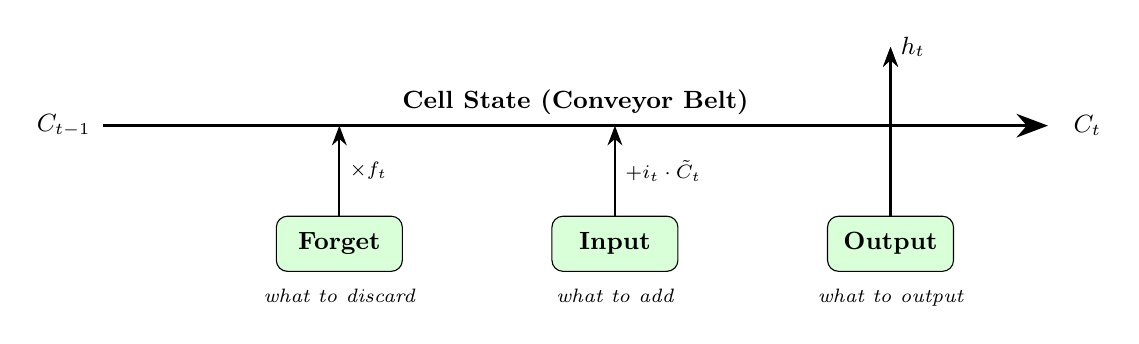
\begin{tikzpicture}[
    gate/.style={draw, rounded corners, fill=green!15, minimum height=0.7cm, minimum width=1.6cm, font=\small\bfseries},
    arr/.style={-{Stealth[length=2.5mm]}, thick},
    lbl/.style={font=\scriptsize\itshape}
]
% Conveyor belt
\draw[very thick, -{Stealth[length=4mm]}] (0, 2) -- node[above, font=\small\bfseries] {Cell State (Conveyor Belt)} (12, 2);
\node[font=\small] at (-0.5, 2) {$C_{t-1}$};
\node[font=\small] at (12.5, 2) {$C_t$};

% Forget gate
\node[gate] (fg) at (3, 0.5) {Forget};
\draw[arr] (fg) -- (3, 2) node[midway, right, lbl] {$\times f_t$};
\node[lbl, below=0.1cm] at (fg.south) {what to discard};

% Input gate
\node[gate] (ig) at (6.5, 0.5) {Input};
\draw[arr] (ig) -- (6.5, 2) node[midway, right, lbl] {$+ i_t \cdot \tilde{C}_t$};
\node[lbl, below=0.1cm] at (ig.south) {what to add};

% Output gate
\node[gate] (og) at (10, 0.5) {Output};
\draw[arr] (10, 2) -- (10, 3);
\draw[arr] (og) -- (10, 3) node[right, font=\small] {$h_t$};
\node[lbl, below=0.1cm] at (og.south) {what to output};
\end{tikzpicture}
\end{center}

\subsection{The Three Gates}

Each gate is controlled by a sigmoid ($\sigma$) that outputs values between 0 and 1.

\subsubsection*{Gate 1: Forget Gate --- \textit{``What old information should I discard?''}}

\begin{equation}
f_t = \sigma(W_f \cdot [h_{t-1}, x_t] + b_f)
\end{equation}

\begin{itemize}[leftmargin=1.5em]
    \item Output near \textbf{0}: forget this information
    \item Output near \textbf{1}: keep this information
\end{itemize}

\textit{Intuition:} When reading ``The cat sat.\ \textbf{The dog} ran'', the forget gate learns to discard information about ``cat'' when the subject changes to ``dog''.

\subsubsection*{Gate 2: Input Gate + Candidate --- \textit{``What new information should I store?''}}

\begin{align}
i_t &= \sigma(W_i \cdot [h_{t-1}, x_t] + b_i) && \text{(how much to add)} \\
\tilde{C}_t &= \tanh(W_C \cdot [h_{t-1}, x_t] + b_C) && \text{(what to add)}
\end{align}

The input gate ($i_t$) decides \textit{how much} new information to add. The candidate ($\tilde{C}_t$) proposes \textit{what} new information to add. Note: sigmoid for the gate (0/1 decision), tanh for the candidate (can be positive or negative).

\subsubsection*{Gate 3: Output Gate --- \textit{``What part of the cell state should I output?''}}

\begin{align}
o_t &= \sigma(W_o \cdot [h_{t-1}, x_t] + b_o) \\
h_t &= o_t \cdot \tanh(C_t)
\end{align}

The output gate filters the cell state to produce the hidden state $h_t$.

\subsection{Cell State Update}

The cell state update is the heart of the LSTM:

\begin{equation}
\boxed{C_t = f_t \cdot C_{t-1} + i_t \cdot \tilde{C}_t}
\end{equation}

Reading this equation:
\begin{itemize}[leftmargin=1.5em]
    \item $f_t \cdot C_{t-1}$: Keep the parts of old memory that the forget gate allows
    \item $i_t \cdot \tilde{C}_t$: Add the parts of new information that the input gate allows
\end{itemize}

\begin{tcolorbox}[intuitionbox={Why This Solves Vanishing Gradients}]
The cell state $C_t$ is updated through \textbf{addition} (not repeated multiplication like in vanilla RNNs). Gradients can flow through the additive path without shrinking, allowing the network to remember information across long sequences.
\end{tcolorbox}

\begin{tcolorbox}[questionbox={Self-Check Q5}]
In an LSTM, what happens to the cell state if the forget gate outputs all 1s and the input gate outputs all 0s? What does this mean in practice? \textit{(Solution in Appendix)}
\end{tcolorbox}

% ============================================================
% 8. GRU
% ============================================================
\section{GRU: Gated Recurrent Unit}

\subsection{Motivation}

LSTMs are powerful but \textbf{complex}: 3 gates, separate cell state and hidden state, many parameters. GRU simplifies this to \textbf{2 gates} and \textbf{merges} the cell state and hidden state into one.

\subsection{The Two Gates}

\subsubsection*{Reset Gate --- \textit{``How much past information to ignore?''}}

\begin{equation}
r_t = \sigma(W_r \cdot [h_{t-1}, x_t] + b_r)
\end{equation}

\begin{itemize}[leftmargin=1.5em]
    \item $r_t \approx 0$: ignore previous hidden state (fresh start)
    \item $r_t \approx 1$: fully use previous hidden state
\end{itemize}

\subsubsection*{Update Gate --- \textit{``How much to keep old state vs.\ adopt new?''}}

\begin{equation}
z_t = \sigma(W_z \cdot [h_{t-1}, x_t] + b_z)
\end{equation}

\begin{itemize}[leftmargin=1.5em]
    \item $z_t \approx 1$: keep previous memory (skip this input)
    \item $z_t \approx 0$: replace with new candidate
\end{itemize}

\subsection{Hidden State Computation}

\textbf{Candidate hidden state:}
\begin{equation}
\tilde{h}_t = \tanh(W \cdot [r_t \odot h_{t-1},\; x_t] + b)
\end{equation}

The reset gate controls how much of the previous hidden state ``leaks'' into the candidate.

\textbf{Final hidden state:}
\begin{equation}
\boxed{h_t = (1 - z_t) \odot h_{t-1} + z_t \odot \tilde{h}_t}
\end{equation}

This is an \textbf{interpolation} between the old hidden state and the new candidate. The update gate $z_t$ simultaneously decides what to forget AND what to add---in LSTM, these are separate decisions.

\subsection{LSTM vs.\ GRU at a Glance}

\begin{center}
\renewcommand{\arraystretch}{1.3}
\begin{tabular}{@{}lcc@{}}
\toprule
\textbf{Feature} & \textbf{LSTM} & \textbf{GRU} \\
\midrule
Gates & 3 (forget, input, output) & 2 (reset, update) \\
States & 2 ($C_t$ + $h_t$) & 1 ($h_t$ only) \\
Parameters & More & Fewer \\
Training speed & Slower & Faster \\
Long sequences & Slightly better & Comparable \\
Small datasets & May overfit & Better generalization \\
\bottomrule
\end{tabular}
\end{center}

\begin{tcolorbox}[questionbox={Self-Check Q6}]
In a GRU, the update gate $z_t$ replaces both the forget gate and input gate of an LSTM. Explain how a single gate can do the job of two. \textit{(Solution in Appendix)}
\end{tcolorbox}

% ============================================================
% 9. SUMMARY
% ============================================================
\section{The Complete Evolution: Summary}

\subsection{Key Equations Reference Card}

\begin{center}
\renewcommand{\arraystretch}{1.5}
\begin{tabular}{@{}p{3cm}p{7cm}p{4.5cm}@{}}
\toprule
\textbf{Model} & \textbf{Core Equation} & \textbf{What it computes} \\
\midrule
\textbf{RNN} & $h_t = \tanh(W_h h_{t-1} + W_x x_t + b)$ & Hidden state \\
\textbf{LSTM Forget} & $f_t = \sigma(W_f [h_{t-1}, x_t] + b_f)$ & What to discard \\
\textbf{LSTM Input} & $i_t = \sigma(W_i [h_{t-1}, x_t] + b_i)$ & What to store \\
\textbf{LSTM Candidate} & $\tilde{C}_t = \tanh(W_C [h_{t-1}, x_t] + b_C)$ & Proposed new content \\
\textbf{LSTM Cell} & $C_t = f_t \cdot C_{t-1} + i_t \cdot \tilde{C}_t$ & Updated cell state \\
\textbf{LSTM Output} & $h_t = o_t \cdot \tanh(C_t)$ & What to output \\
\textbf{GRU Reset} & $r_t = \sigma(W_r [h_{t-1}, x_t] + b_r)$ & How much past to use \\
\textbf{GRU Update} & $z_t = \sigma(W_z [h_{t-1}, x_t] + b_z)$ & Keep old vs.\ use new \\
\textbf{GRU Hidden} & $h_t = (1{-}z_t) h_{t-1} + z_t \tilde{h}_t$ & Interpolated state \\
\bottomrule
\end{tabular}
\end{center}

\subsection{What Comes Next: Transformers}

All RNN-based architectures share three fundamental limitations:

\begin{enumerate}[leftmargin=1.5em]
    \item \textbf{Encoding bottleneck} --- the entire sequence is compressed into a fixed-size vector
    \item \textbf{No parallelization} --- tokens must be processed one by one (sequential)
    \item \textbf{Limited long-range memory} --- even LSTMs struggle with very long sequences
\end{enumerate}

Transformers (Vaswani et al., 2017, \textit{``Attention is All You Need''}) solve all three by replacing recurrence with \textbf{self-attention}, enabling parallel processing of all tokens simultaneously. This is the subject of Lecture~5.

\begin{tcolorbox}[questionbox={Self-Check Q7}]
What is the fundamental architectural difference between RNN-based models and Transformers that allows Transformers to process sequences in parallel? \textit{(Solution in Appendix)}
\end{tcolorbox}

% ============================================================
% APPENDIX
% ============================================================
\newpage
\section*{Appendix: Solutions to Self-Check Questions}
\addcontentsline{toc}{section}{Appendix: Solutions to Self-Check Questions}

\subsection*{Q1: Why can't we feed variable-length sequences without padding?}

In theory, a single RNN can handle variable-length sequences because it processes one token at a time. However, in practice, we process data in \textbf{batches} for computational efficiency. A batch is represented as a matrix (\texttt{batch\_size} $\times$ \texttt{sequence\_length}), and matrices require all rows to have the same number of columns. Padding ensures all sequences have uniform length, enabling efficient GPU-based parallel computation across the batch. Without padding, we would need to process each sequence individually (batch size = 1), which is approximately $N$ times slower.

\subsection*{Q2: Would ``AI like I'' produce the same $h_3$?}

\textbf{No.} The RNN processes words sequentially, and the hidden state at each step depends on the previous hidden state. Changing the word order changes what information the hidden state carries at each step:

\begin{itemize}[leftmargin=1.5em]
    \item ``I like AI'': $h_1$ encodes ``I'', $h_2$ encodes ``I + like'', $h_3$ encodes ``I + like + AI''
    \item ``AI like I'': $h_1$ encodes ``AI'', $h_2$ encodes ``AI + like'', $h_3$ encodes ``AI + like + I''
\end{itemize}

Even though the same words are processed, the \textbf{context accumulation} differs because the hidden state is built incrementally. This is precisely how RNNs capture word order, unlike bag-of-words models.

\subsection*{Q3: Why sigmoid for gates, not tanh?}

Gates act as \textbf{binary switches}---they decide how much information to keep~(1) or discard~(0). Sigmoid outputs values in $[0, 1]$, which naturally represents a ``percentage'' of information to pass through.

If we used tanh (range $[-1, +1]$) for the forget gate, a value of $-1$ would \textbf{negate} the cell state (flip its sign), not forget it. Negative values would \textbf{distort} stored information instead of discarding it. Sigmoid ensures the gate behaves like a \textbf{valve}: 0 = fully closed, 1 = fully open, 0.5 = keep half.

\subsection*{Q4: Can a vanilla RNN use word~1 at word~100?}

\textbf{Effectively no.} The gradient signal from word~100 back to word~1 involves multiplying $W_h$ approximately 99 times. If the largest eigenvalue is, say, 0.9:
\[
0.9^{99} \approx 0.00003
\]
The gradient shrinks to near zero, meaning updates to the weights based on the relationship between word~1 and word~100 are negligibly small. The network effectively ``forgets'' word~1 by the time it reaches word~100.

\subsection*{Q5: Forget gate = all 1s, input gate = all 0s?}

The cell state update becomes:
\[
C_t = 1 \cdot C_{t-1} + 0 \cdot \tilde{C}_t = C_{t-1}
\]
The cell state is \textbf{passed through unchanged}---no old information is forgotten, and no new information is added. In practice, this means the LSTM is choosing to \textbf{completely preserve its current memory} and ignore the current input. This is useful when processing irrelevant tokens (e.g., stop words like ``the'' or ``a'') while tracking a long-distance dependency.

\subsection*{Q6: How does one GRU gate replace two LSTM gates?}

In LSTM, the forget and input gates operate \textbf{independently}. In GRU, the update gate \textbf{couples} them:
\[
h_t = (1 - z_t) \cdot h_{t-1} + z_t \cdot \tilde{h}_t
\]

\begin{itemize}[leftmargin=1.5em]
    \item $z_t = 1$: fully adopt new candidate (input=1, forget=0)
    \item $z_t = 0$: fully keep old state (input=0, forget=1)
\end{itemize}

The constraint is: \textbf{the amount you forget equals the amount you replace}. LSTM can independently control forgetting and adding, while GRU assumes they are complementary. This works well in practice while reducing parameters.

\subsection*{Q7: What allows Transformers to parallelize?}

RNNs are inherently \textbf{sequential}: computing $h_t$ requires $h_{t-1}$, which requires $h_{t-2}$, and so on. Each token must wait for all previous tokens.

Transformers replace recurrence with \textbf{self-attention}, which computes relationships between \textbf{all pairs of tokens simultaneously} via matrix multiplication. All token representations can be computed \textbf{in parallel}, making Transformers dramatically faster on GPU hardware. The trade-off is $O(n^2)$ memory for the attention matrix, but the parallelization speedup far outweighs this cost.

\end{document}
